\begin{figure*}
\centering
	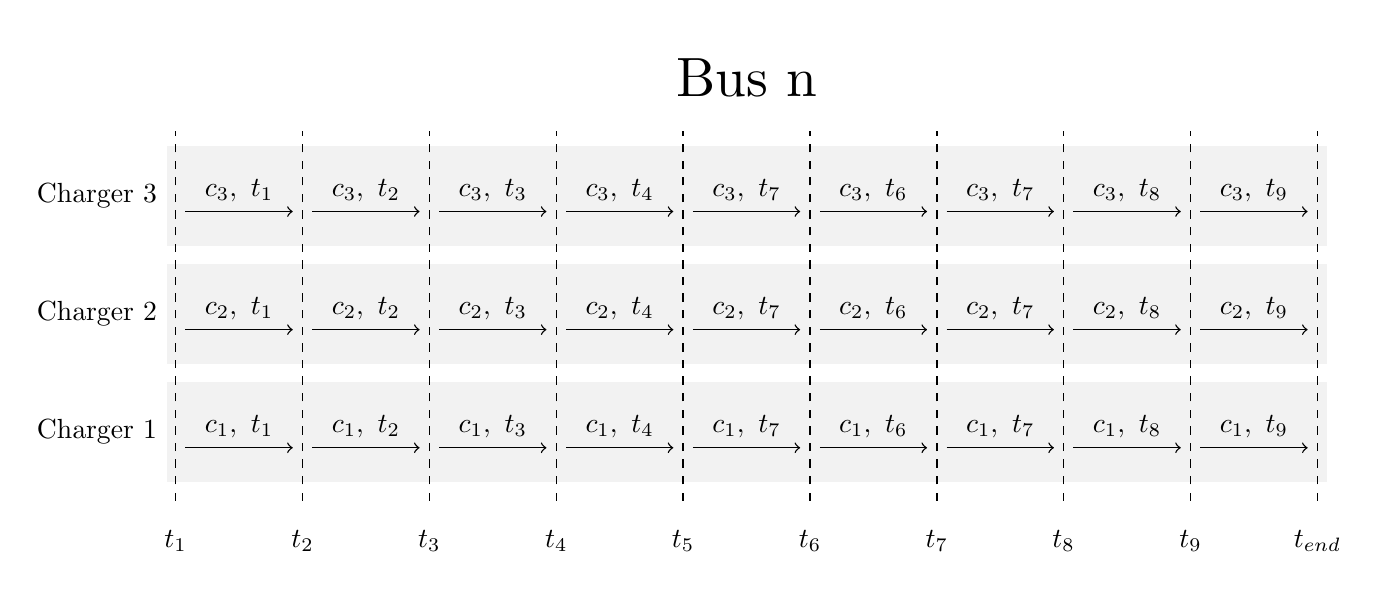
\begin{tikzpicture}
		\node[rectangle, minimum width=5.8in, minimum height=0.5in](title) at (7.75, 5.5){\scalebox{2}{Bus n}};
		\node[rectangle, fill=gray!10, minimum width=5.8in, minimum height=0.5in](bus1Box) at (7.75,1){};
		\node(bus1BoxLabel) at (-0.5, 1){Charger 1}; 
		
		\node[rectangle, fill=gray!10, minimum width=5.8in, minimum height=0.5in](bus2Box) at (7.75,2.5){};
		\node(bus1BoxLabel) at (-0.5, 2.5){Charger 2};
		
		\node[rectangle, fill=gray!10, minimum width=5.8in, minimum height=0.5in](bus3Box) at (7.75,4){};
		\node(bus1BoxLabel) at (-0.5, 4){Charger 3};
		
		\foreach \curLab/\preLab[count=\c, evaluate=\c as \pos using {0.5 + (\c - 1)*14.5/9}] in {t_1/t_1, t_2/t_1, t_3/t_2, t_4/t_3, t_5/t_4, t_6/t_7, t_7/t_6, t_8/t_7, t_9/t_8, t_{end}/t_9}
		{
			\node[label=below:$\curLab$](b) at (\pos, 0){};
			\node(t) at (\pos, 4.7){};
			\draw[dashed, line width=0.5pt] (b.north) -- (t.north); 
			\ifnum\c>1 
				\node(b1Curr) at (\pos, 1   - 0.2){};
			\node(b2Curr) at (\pos, 2.5 - 0.2){};
			\node(b3Curr) at (\pos, 4   - 0.2){};
			\draw[->, line width=0.5pt] (b1Prev.east) -- node[midway, above]{$c_1,\ \preLab$}(b1Curr.west);
			\draw[->, line width=0.5pt] (b2Prev.east) -- node[midway, above]{$c_2,\ \preLab$}(b2Curr.west);
			\draw[->, line width=0.5pt] (b3Prev.east) -- node[midway, above]{$c_3,\ \preLab$}(b3Curr.west);	
			\fi
				\node(b1Prev) at (\pos, 1   - 0.2){};
			\node(b2Prev) at (\pos, 2.5 - 0.2){};
			\node(b3Prev) at (\pos, 4   - 0.2){};	
		}
	\end{tikzpicture}
	\caption{Description of the bus and time axis}
	\label{fig:layout}
\end{figure*}

